% FitDash — Training Copilot: abstracted architecture graph (standalone).
% Build:  latexmk -pdf fitdash-architecture-graph-abstract.tex
\documentclass[border=12pt]{standalone}
\usepackage[T1]{fontenc}
\usepackage[sfdefault]{FiraSans}
\usepackage{xcolor}
\usepackage{tikz}
\usetikzlibrary{positioning,arrows.meta,fit,backgrounds,calc}

\definecolor{fdNavy}{HTML}{0B1219}
\definecolor{fdSlate}{HTML}{16212B}
\definecolor{fdBorder}{HTML}{1E293B}
\definecolor{fdTeal}{HTML}{2DD4BF}
\definecolor{fdTealDark}{HTML}{14B8A6}

\begin{document}
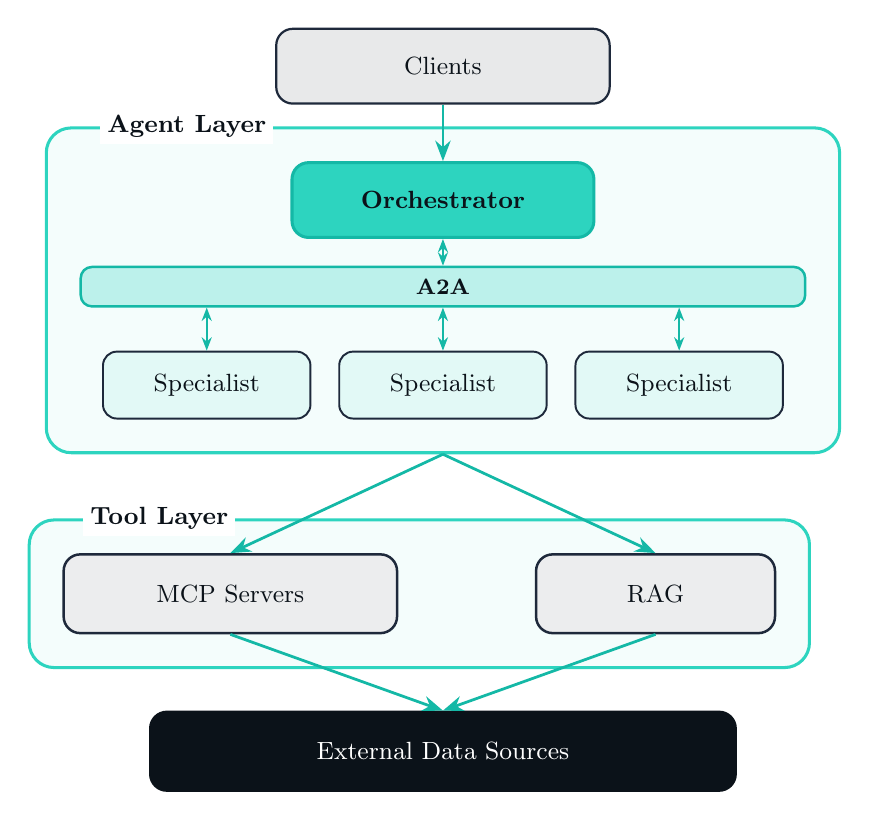
\begin{tikzpicture}[
  font=\sffamily,
  box/.style={rounded corners=6pt, draw=fdBorder, line width=0.8pt, fill=fdSlate!10,
              text=fdNavy, align=center, font=\small, minimum height=0.95cm},
  orch/.style={rounded corners=6pt, draw=fdTealDark, line width=1.1pt, fill=fdTeal,
               text=fdNavy, align=center, font=\small\bfseries, text width=3.6cm, minimum height=0.95cm},
  agent/.style={rounded corners=5pt, draw=fdBorder, line width=0.7pt, fill=fdTeal!14,
                text=fdNavy, align=center, font=\small, text width=2.4cm, minimum height=0.85cm},
  bus/.style={rounded corners=4pt, draw=fdTealDark, line width=0.9pt, fill=fdTeal!32,
              text=fdNavy, font=\footnotesize\bfseries, minimum width=9.2cm, minimum height=0.5cm},
  comp/.style={rounded corners=6pt, draw=fdBorder, line width=0.9pt, fill=fdSlate!8,
               text=fdNavy, align=center, font=\small, minimum height=1.0cm},
  ext/.style={rounded corners=6pt, draw=fdNavy, line width=0.9pt, fill=fdNavy,
              text=white, align=center, font=\small, minimum height=1.0cm},
  group/.style={rounded corners=9pt, draw=fdTeal, line width=1.1pt, fill=fdTeal!5, inner sep=12pt},
  ltitle/.style={font=\bfseries\small, text=fdNavy, fill=white, inner sep=2.5pt},
  flow/.style={-{Stealth[length=2.6mm]}, line width=1.0pt, draw=fdTealDark},
  link/.style={{Stealth[length=1.7mm]}-{Stealth[length=1.7mm]}, line width=0.8pt, draw=fdTealDark},
]

% Clients
\node[box, text width=4cm] (clients) at (0,0) {Clients};

% Agent layer
\node[orch] (orch) at (0,-1.7) {Orchestrator};
\node[bus]  (bus)  at (0,-2.8) {A2A};
\node[agent] (a1) at (-3,-4.05) {Specialist};
\node[agent] (a2) at ( 0,-4.05) {Specialist};
\node[agent] (a3) at ( 3,-4.05) {Specialist};
\draw[link] (orch.south) -- (orch.south |- bus.north);
\foreach \a in {a1,a2,a3}{ \draw[link] (\a.north) -- (\a.north |- bus.south); }

% Tool layer
\node[comp, text width=4.0cm] (mcp) at (-2.7,-6.7) {MCP Servers};
\node[comp, text width=2.8cm] (rag) at ( 2.7,-6.7) {RAG};

% Data
\node[ext, text width=7.2cm] (data) at (0,-8.7) {External Data Sources};

% Grouping boxes
\begin{scope}[on background layer]
  \node[group, fit=(orch)(bus)(a1)(a3)] (AL) {};
  \node[group, fit=(mcp)(rag)] (TL) {};
\end{scope}
\node[ltitle, anchor=west] at ($(AL.north west)+(0.7,0)$) {Agent Layer};
\node[ltitle, anchor=west] at ($(TL.north west)+(0.7,0)$) {Tool Layer};

% Flows
\draw[flow] (clients) -- (orch);
\draw[flow] (AL.south) -- (mcp.north);
\draw[flow] (AL.south) -- (rag.north);
\draw[flow] (mcp.south) -- (data.north);
\draw[flow] (rag.south) -- (data.north);

\end{tikzpicture}
\end{document}
